\documentclass[12pt,reqno]{amsart}
\usepackage{./header, amssymb}

\hdr{Mathematical Statistics}{Chapter 13: Learning}

\begin{document}

\bigskip

\prob Consider a \textit{Naive Bayes model} as described in the programming assignment for chapter 12. The underlying graph is of the form

\bigskip
\begin{center}
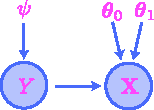
\includegraphics[scale=1.5]{nb}
\end{center}
\bigskip

where $\mathbf{X} \in \mathbb{R}^n$. The parameters are given by a number $\psi\in [0,1]$ which parametrizes the distribution of $Y\sim \mathcal{B}er(\psi)$, as well as two vectors $\boldsymbol{\theta}_0, \boldsymbol{\theta}_1 \in [0,1]^n$. The link function at $\mathbf{X}$ is given by
	\[
	p(\mathbf{x} \mid y ; \  \boldsymbol{\theta}_0, \boldsymbol{\theta}_1 ) = \prod_{j=1}^n \phi_j^{x_j}(1-\phi_j)^{1-x_j}
	\]
where
	\[
	\boldsymbol{\phi} = (1-y) \boldsymbol{\theta}_0 + y \boldsymbol{\theta}_1
	\]
and	$\boldsymbol{\phi}^\intercal = (\phi_1,\ldots,\phi_n)$.

\bigskip
\begin{enumerate}
\item Assuming that Naive Bayes models are trained as \textbf{generative} models, write down a formula for the model likelihood function $\mathcal{L}_\text{model}(\psi,\boldsymbol{\theta}_0,\boldsymbol{\theta}_1)$. For simplicity, your formula should contain the $\phi_j$'s rather than the parameters $\boldsymbol{\theta}_0$ and $\boldsymbol{\theta}_0$ themselves.\vfill
\item Using your answer from part (a), write down a formula for the model surprisal function $\mathcal{I}_\text{model}(\psi,\boldsymbol{\theta}_0,\boldsymbol{\theta}_1)$. For simplicity, your formula should contain the $\phi_j$'s rather than the parameters $\boldsymbol{\theta}_0$ and $\boldsymbol{\theta}_0$ themselves.\vfill
\item Using your answer from part (b), write down an explicit formula for the cross entropy stochastic objective function $J(\psi,\boldsymbol{\theta}_0,\boldsymbol{\theta}_1)$ for a dataset of size $m$.\vfill
\end{enumerate}








\newpage
\prob Consider the observed dataset
	\[
	(0, 0), (1, 1), (2,3) \in \mathbb{R}^2.
	\]
Using this dataset, compute the exact MLEs for the parameters $\beta_0$ and $\beta_1$ of a simple linear regression model (with known variance).

\vfill
\prob For the neural network trained in Section 13.5, compute the following:

\bigskip
\begin{enumerate}
\item The number of gradient steps per epoch.\vfill
\item The \textit{exact} number of gradient steps over all epochs.\vfill
\item The number of trainable parameters in the network.\vfill
\end{enumerate}

\end{document}